\RequirePackage{luatex85}
\documentclass{standalone}

\usepackage{fontspec, unicode-math}
\setsansfont[Scale=MatchLowercase]{TeX Gyre Heros}
\setmathfont{TeX Gyre Termes Math}

\usepackage{tikz}
\usetikzlibrary{shapes.multipart}

\tikzset{
  every picture/.style={font={\sffamily\normalsize}, >=stealth},
  every pin edge/.style={black}}

\begin{document}

  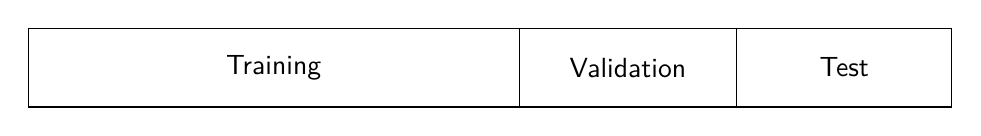
\begin{tikzpicture}
    \node [rectangle split,
           rectangle split horizontal,
           rectangle split parts=3,
           draw,
           minimum height=1cm,
           align=center]
    {
      \nodepart[text width=6cm]{one}Training
      \nodepart[text width=2.5cm]{two}Validation
      \nodepart[text width=2.5cm]{three}Test
    };
  \end{tikzpicture}

\end{document}
